\section{Areas in the Plane}
\begin{lemma}
	If $f(x) \geq g(x)$ on $[a,b]$ then the area between $f(x)$ and $g(x)$ on $[a,b]$ is given by
	\begin{equation*}
		A = \int_{a}^{b}{\left(f(x)-g(x)\right)\d{x}}.
	\end{equation*}
\end{lemma}
\noindent
You can easily visualize why this is true.
We can break the integral into two parts: adding the area under $f$ and the other subtracting the area under $g$.
The first integral will over count the area between $f$ and $g$, counting all area between $f$ and the $x$-axis.
The second integral will subtract exactly the amount of area that is over counted: the area that is also between $g$ and the $x$-axis.

\begin{figure}[H]
	\label{area_between_curves}
	\centering
	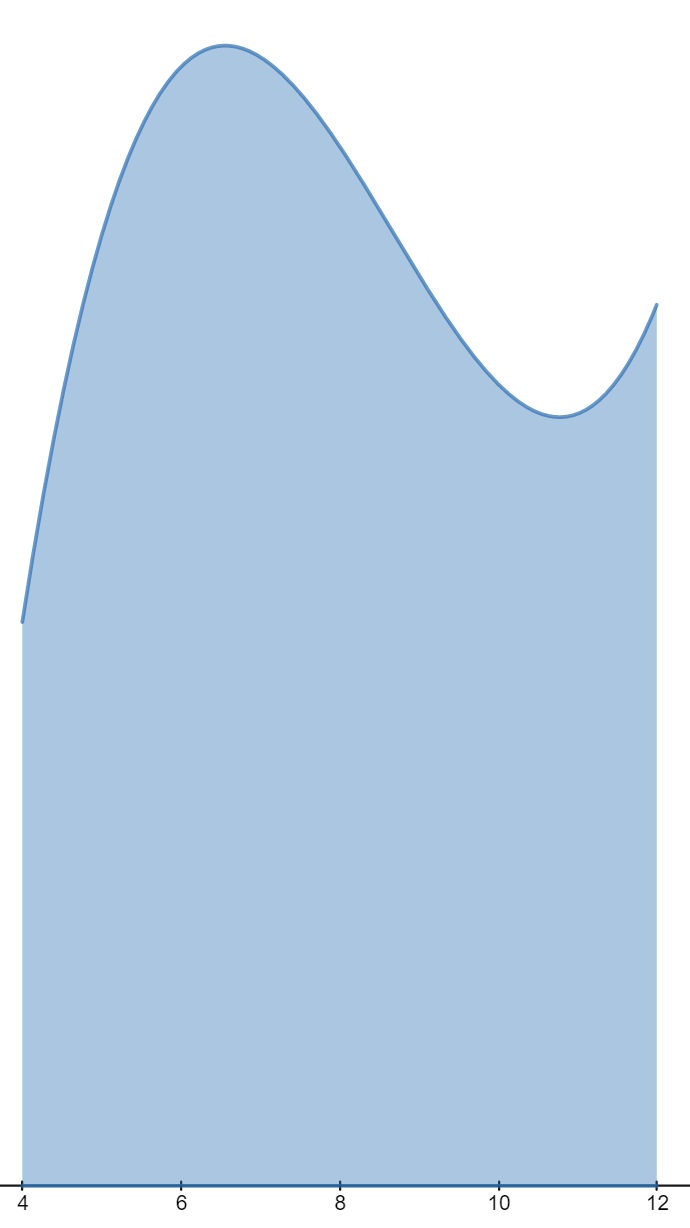
\includegraphics[width = 0.33\textwidth]{./applications_integrals/curve1.png}
	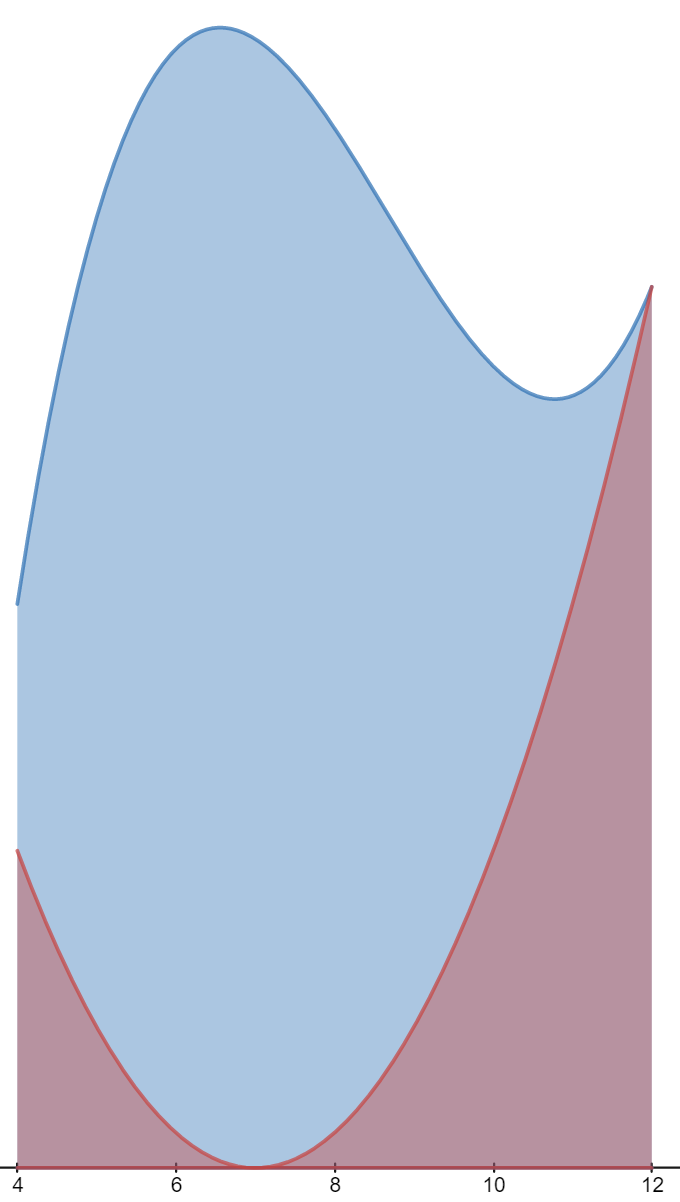
\includegraphics[width = 0.33\textwidth]{./applications_integrals/curve2.png}
	\caption{\hyperref{}{}{}{Subtracting two areas to get the area between them}}
\end{figure}
\noindent
Even if both of the curves has more area below the $x$-axis, the same idea applies.
$f$ will give a smaller-magnitude negative area, while $g$ will give a larger magnitude negative area.
Subtracting a larger-magnitude negative number from a smaller magnitude negative number will give a positive area.

\begin{example}
	Find the area enclosed between the two curves $y=2-x^2$ and $y=-x$.
\end{example}
These two curves intersect at $x=-1$ and $x=2$.
Applying the formula,
\begin{align*}
	A &= \int_{-1}^{2}{((2-x^2)-(-x))\d{x}} \\
	&= 2x-\frac{x^3}{3} + \frac{x^2}{2}\biggr\rvert_{-1}^{2} \\
	&= \frac{9}{2}.
\end{align*}

\subsection{Subregions}
Sometimes it might be useful to break the enclosed regions into subregions and find the area of each separately.
\begin{example}
	Find the area above the $x$-axis, below $y=\sqrt{x}$, and above $y=x-2$.
\end{example}
If we simply took the area between the two curves, we'd count some area we don't want beneath the $x$-axis\footnote{Although this extra region is just a triangle and not too hard to find the area of, you'd effectively be applying the same strategy of two subregions, they'd just overlap. However, using geometry to your advantage is certainly a valid approach.}.
Instead, we can break the area into two subregions: one between the $x$-axis and $\sqrt{x}$ and the other between $x-2$ and $\sqrt{x}$.
\begin{figure}[H]
	\label{subregions}
	\centering
	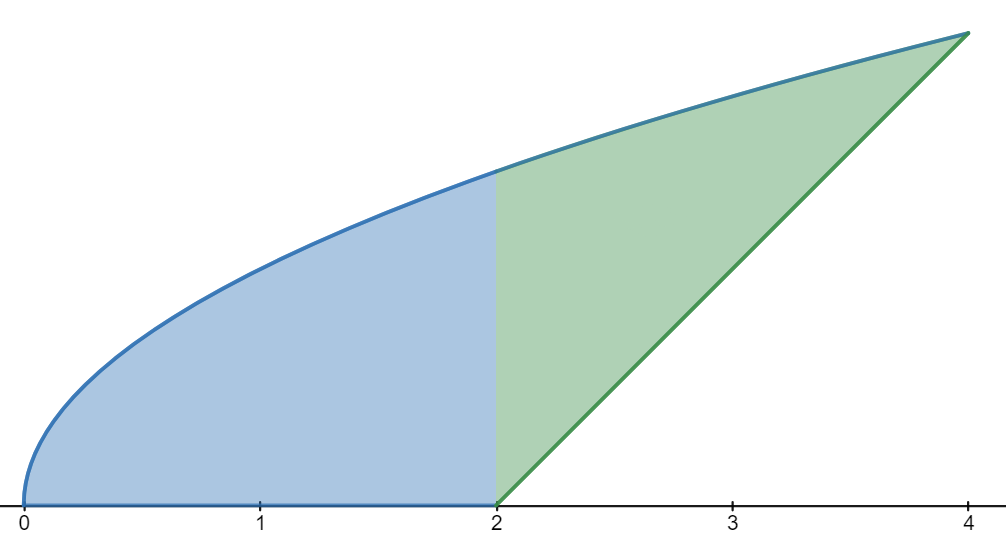
\includegraphics[width = 0.33\textwidth]{./applications_integrals/two_regions.png}
	\caption{\hyperref{}{}{}{Break complicated areas into simpler subregions}}
\end{figure}
\indent
Finding the area of the blue region,
\begin{equation*}
	A_1 = \int_{0}^{2}{\sqrt{x}\d{x}} = \frac{2x\sqrt{x}}{3}\biggr\rvert_0^2 = \frac{4\sqrt{2}}{3}.
\end{equation*}
\indent
Finding the area of the green region,
\begin{equation*}
	A_2 = \int_{2}^{4}{(\sqrt{x}-(x-2))\d{x}} = \frac{2x\sqrt{x}}{3} - \frac{x^2}{2} + 2x \biggr\rvert_2^4 = \frac{10}{3} - \frac{4\sqrt{2}}{3}.
\end{equation*}
\indent
Adding the areas of the two regions,
\begin{equation*}
	A = A_1 + A_2 = \frac{10}{3}.
\end{equation*}

\subsection{Integrating with Respect to $y$}
Another strategy when finding the area of more complex regions is to see if they become easier to deal with if we were to instead integrate with respect to $y$.
In the above example, it is indeed easier to work with respect to $y$ because both bounding curves are between the same $y$ values.
\begin{example}
	Find the area above the $x$-axis, below $y=\sqrt{x}$, and above $y=x-2$.
\end{example}
We need to rearrange our equations to be of the form $x=\ldots$ instead of $y=\ldots$ by simply solving for $x$.
\begin{equation*}
	x = y^2, y\geq 0 \text{ and } x = y+2.
\end{equation*}
\indent
Since $x=y+2$ is further from the $x$-axis, it becomes our top curve.
\begin{align*}
	A &= \int_{0}^{2}{((y+2)-y^2)\d{y}} \\
	&= \frac{y^2}{2} + 2y - \frac{y^3}{3} \biggr\rvert_0^2 \\
	&= \frac{10}{3}.
\end{align*}